\chapter{Introduction}
%Ziel des Versuchs.
Aim of this experiment is to examin the statistical characteristics of radioactive decay as well as comparing the expected
with the actual behavior of the core component - the \textsc{Geiger-Müller}-Tube (GMT).\par
A GMT is a device to detect and quantify radiation by counting induced ionization events inside its volume. The nature
of the GMT does not allow to distinguish between types of sources of ionization directly (i.e. \(\alpha\)-,
\(\beta\)- or \(\gamma\)-radiation).\par\medskip
%
%
\section{Half-life time}
Radioactive decay is a statistical process. According to quantum physics it is impossible to predict the life span of a
single atom. Given a significantly large number of atoms one can state the overall time until half of the nuclei present
at \(t_0\) did disintegrate. Thus, for each radioactive nuclide one can describe a characteristical mean lifespan \(\tau\)\cite{Eichler.2016}\cite{Papula.MatheIngenieure.2018}.\par
Mathmatically speaking, the amount of decayed radio-nuclides after a time \(t\) can be described as \cref{eq:zerfallsgesetz}.
%
\begin{equation}
    \dot{N}(t) = -\tau N(t) \quad \Leftrightarrow \quad N(t) = N_0 e^{-\nicefrac{t}{\tau}}
    \label{eq:zerfallsgesetz}
\end{equation}
%
If \(\frac{1}{2}N_0 = N(t)\) is inserted in above equation and solved in terms of the time \(t\) one gets the half-life \(T_{\nicefrac{1}{2}}\)
with
%
\begin{equation}
    T_{\nicefrac{1}{2}} = \frac{\ln2}{\tau}
    \label{eq:halflife}
\end{equation}
%
%
\section{GMT-characteristics}
%
%
The GMT's principle of operation is based around the phenomenon called \textsc{Townsend}-discharge. If the seperated
particles after an ionising event are left with enough kinetic energy, they become ionising themself striking surrounding
atoms. This releases a cascade of free electrons and positive nuclei according to \cref{fig:avalanche_discharge}.
\begin{figure}[h]
    \centering
    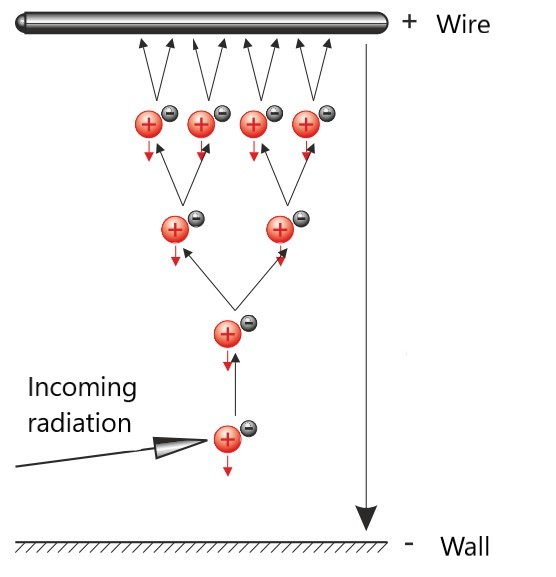
\includegraphics[width=.4\textwidth]{referenzen/scheme_avalanche.jpg}
    \caption{A single ionising event releases an avalanche of free electrons. These - fast enough accelerated toward the anode - form a pulse that can be further processed \cite{Eichler.2016}.}
    \label{fig:avalanche_discharge}
\end{figure}
To prevent the \(e^-\) to recombine before they reach the anode the accelerating voltage needs to be high enough. On the
other hand a voltage too high leads to spontanious self discharge of the inert gas. A rapid rise of counts can be observed
covering the actual ionisation events.
\begin{figure}[h]
    \centering
    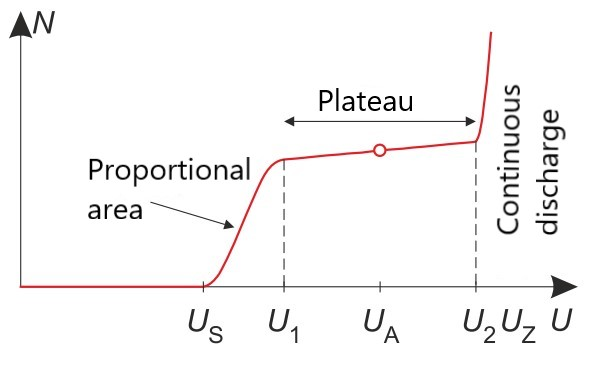
\includegraphics[width=.5\textwidth]{referenzen/gmt_plot.jpg}
    \caption[Characteristical curve of a GMT]{The characteristical curve of a GM-Tube. At a onset-voltage \(U_S\) the count rate is rapidly rising (plateau area). A certain voltage-range 
    is considered the working area (plateau). Further increase of the acceleration voltage leads to a second steep rise of counts (continuous discharge) \cite{Eichler.2016}.}
\end{figure}
%
%
While the preceding avalanche is not yet expired a new event will produce no pulses, hence, no counts can be measured.
This dead time is usually within the range of \(\SI{10^{-4}}{s}\). Still, the sensitivity of the GMT does not instantaniously
recover to full potential. Instead, for another period of time ongoing pules will gradually rise in magnitude until reaching
there original (maximum) level. In consequence some pulses may be too small for the downstream amplifying electronics to
trigger ultimately leading to undesired false-negatives i.e. too low count rate in a highly radiating environment.\par
%
%
\section{Stochastic principles}
Since radioactive decay is a stochastic process, some usefull mathmatic principles need to be discussed.
\subsection{Binomial distribution}
\begin{quote}
    A random experiment with only \textit{two mutually exclusive} results is called \textit{Bernoulli-experiment}\cite{Papula.MatheFormelsammlung.2017}
\end{quote}
Given an event has only two possible outcomes - \(A\) or \(\bar{A}\) - with the individual propabilities \(p(A) = 1 - p(\bar{A})\)
one can express the propability \(P\) for \(k\) successive events \(A\) within \(n\) repetitions as follows:
\begin{equation}
    P(k) = \binom{n}{k} \cdot p(A)^k \cdot p(\bar{A})^{n-k}
    \label{eq:wahrscheinlichkeitsfunktion}
\end{equation}
Accordingly, the propability for \(k \leq x\) outcomes is expressed as
\begin{equation}
    P(k \leq x) = \sum_{k \leq x} \binom{n}{k}p(A)^k \cdot (1-p(A))^{n-k}
\end{equation}